% Flowchart
% Author: Stefan Kottwitz
% https://www.packtpub.com/hardware-and-creative/latex-cookbook
\documentclass[border=20pt]{standalone}
%\usepackage[a0paper,vmargin=3cm]{geometry}
\usepackage[a4paper,vmargin=3cm]{geometry}
%\usepackage{cooltooltips]
%\usepackage{hyperref}
%
%\usepackage{xcolor}
%
%\usepackage{pdfcomment}



\usepackage{tikz}
\usetikzlibrary{matrix,calc,shapes}
\tikzset{
  treenode/.style = {shape=rectangle, rounded corners,
	draw, anchor=center,
	text width=12em, align=center,
	top color=white, bottom color=blue!20,
	inner sep=1ex},
%  decision/.style = {treenode, diamond, inner sep=0pt},
  %concept/.style = {treenode, diamond, inner sep=0pt},
  concept/.style = {treenode, bottom color=cyan!30},
  blank/.style = {draw=none, bottom color=white!30, font=\ttfamily\large},
  background/.style      = {treenode, bottom color=red!30},
  %background/.style      = {treenode, bottom color=red!30, font=\ttfamily\small},
  section/.style      = {treenode, bottom color=green!30},
  activity/.style = {treenode, bottom color=yellow!30},
  skill/.style = {treenode, bottom color=blue!30},
  topic/.style = {treenode, bottom color=orange!30},
  root/.style     = {treenode, font=\Large, bottom color=yellow!30},
%  env/.style      = {treenode, font=\ttfamily\normalsize},
  finish/.style   = {root, bottom color=green!40},
  dummy/.style    = {circle,draw}
}
\newcommand{\yes}{edge node [above] {yes}}
\newcommand{\no}{edge  node [left]  {no}}
\begin{document}

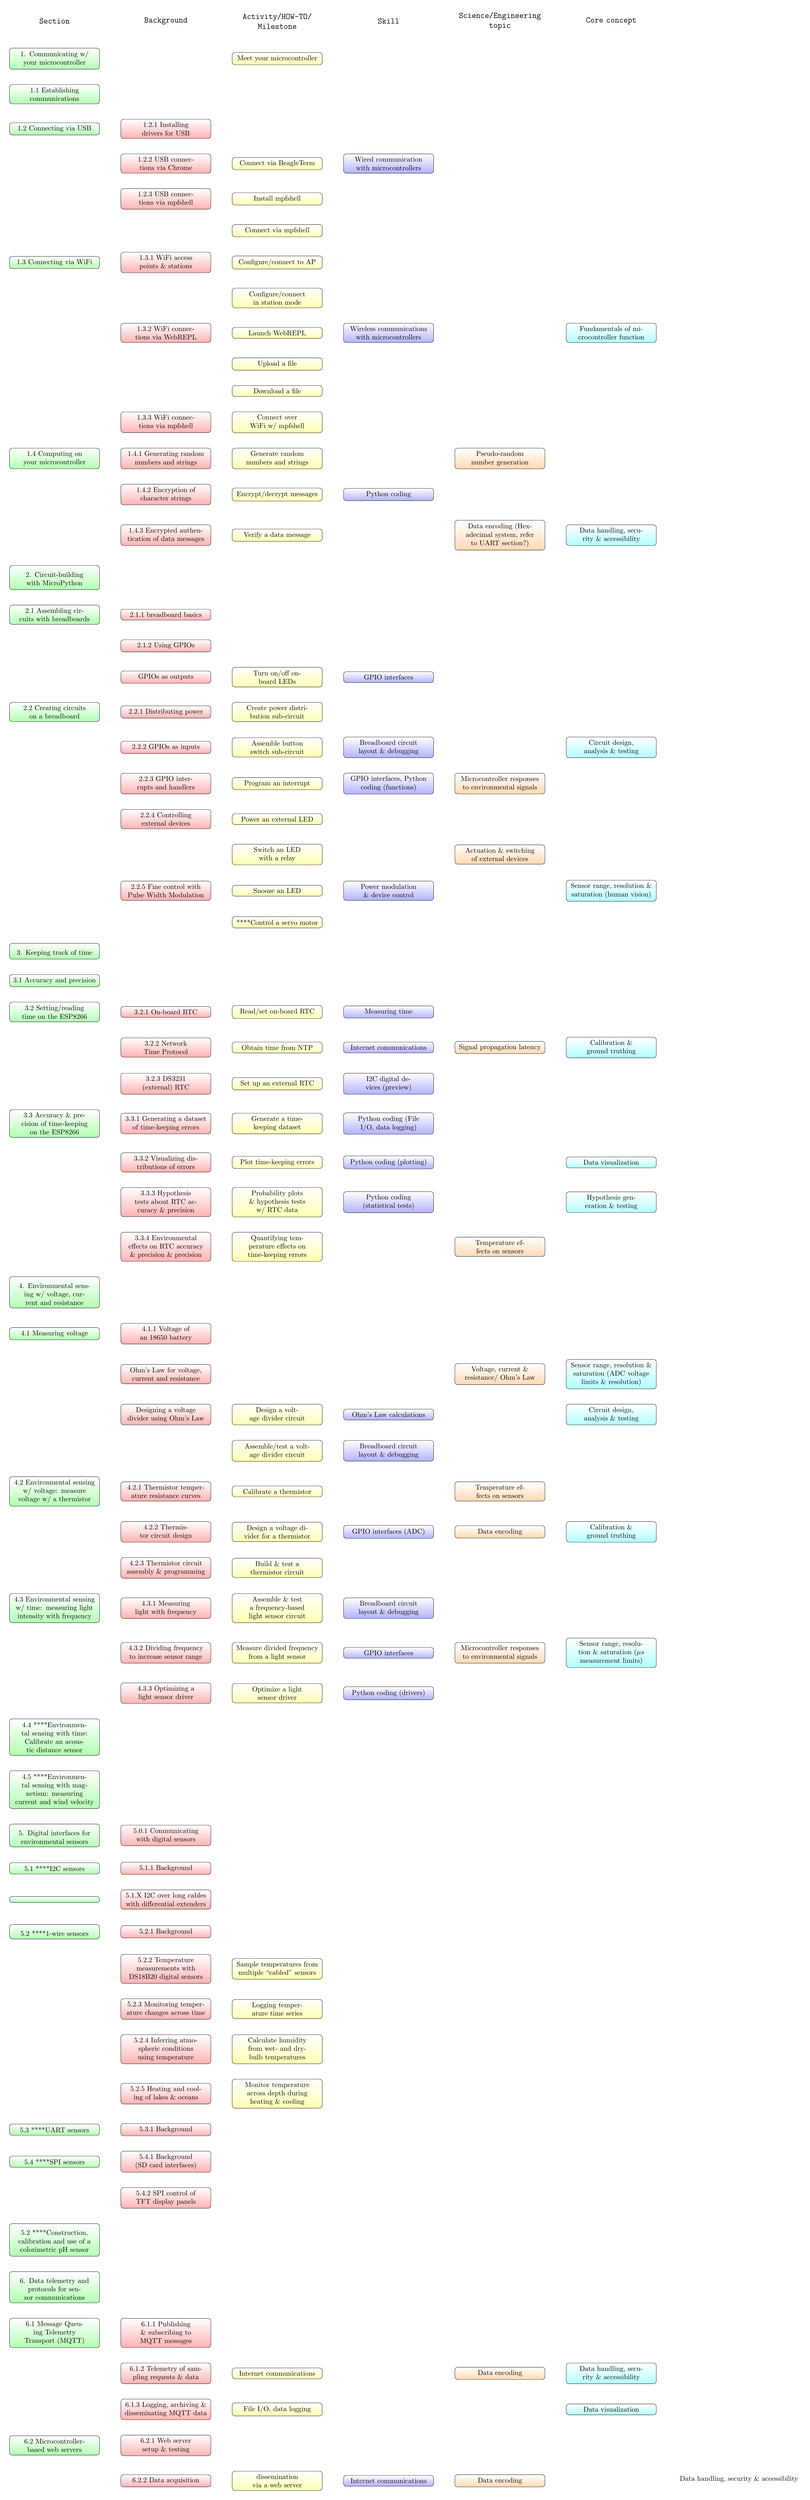
\begin{tikzpicture}[-latex]
  \matrix (chart)
    [
      matrix of nodes,
      column sep      = 3em,
      row sep         = 5ex,
      column 1/.style = {nodes={section}},
      column 2/.style = {nodes={background}},
      column 3/.style = {nodes={activity}},
	    column 4/.style = {nodes={skill}},
      column 5/.style = {nodes={topic}},
	    column 6/.style = {nodes={concept}}
%      column 7/.style = {nodes={concept}},
%	  column 8/.style = {nodes={section}},
%	  column 9/.style = {nodes={background}}
    ]
    {
      %& &  |[root]| Prosection               \\
      |[blank]|Section     & |[blank]|Background  & |[blank]|Activity/HOW-TO/ Milestone  & |[blank]|Skill &  |[blank]|Science/Engineering topic & |[blank]|Core concept  \\
      1. Communicating w/ your microcontroller   & & Meet your microcontroller     & &        &      \\
      1.1 Establishing communications    &  &    & &        &      \\
      1.2 Connecting via USB    & 1.2.1 Installing drivers for USB &    & &        &      \\
          & 1.2.2 USB connections via Chrome & Connect via BeagleTerm & Wired communication with microcontrollers &        &      \\
          & 1.2.3 USB connections via mpfshell &   Install mpfshell & &        &      \\
          &  &   Connect via mpfshell & &        &      \\
      1.3 Connecting via WiFi     & 1.3.1 WiFi access points \& stations &  Configure/connect to AP  &  &        &      \\
                                 &   &  Configure/connect in station mode  & &        &      \\
           & 1.3.2 WiFi connections via WebREPL &  Launch WebREPL  & Wireless communications with microcontrollers &        & Fundamentals of microcontroller function     \\
                                 &   &  Upload a file  & &        &      \\
                                 &   &  Download a file  & &        &      \\
           & 1.3.3 WiFi connections via mpfshell & Connect over WiFi w/ mpfshell  & &        &      \\
      1.4 Computing on your microcontroller    &  1.4.1 Generating random numbers and strings &  Generate random numbers and strings  & & Pseudo-random number generation         &      \\
          & 1.4.2 Encryption of character strings &  Encrypt/decrypt messages  & Python coding &        &  \\
          & 1.4.3 Encrypted authentication of data messages &  Verify a data message  & &  Data encoding (Hexadecimal system, refer to UART section?)    &  Data handling, security \& accessibility    \\

      2. Circuit-building with MicroPython   &  &    & &        &      \\
      2.1 Assembling circuits with breadboards    & 2.1.1 breadboard basics &    & &        &      \\
          & 2.1.2 Using GPIOs &    & &        &      \\
          &  GPIOs as outputs &  Turn on/off on-board LEDs  & GPIO interfaces &        &      \\
      2.2 Creating circuits on a  breadboard   & 2.2.1 Distributing power & Create power distribution sub-circuit   & &        &      \\
         & 2.2.2 GPIOs as inputs & Assemble button switch sub-circuit   & Breadboard circuit layout \& debugging &        &  Circuit design, analysis \& testing   \\
         & 2.2.3 GPIO interrupts and handlers & Program an interrupt   & GPIO interfaces, Python coding (functions) &  Microcontroller responses to environmental signals      &      \\
         & 2.2.4 Controlling external devices & Power an external LED   & &        &      \\
         &  & Switch an LED with a relay   &  &  Actuation \& switching of external devices      &      \\
         & 2.2.5 Fine control with Pulse Width Modulation & Snooze an LED   & Power modulation \& device control &        & Sensor range, resolution \& saturation (human vision) \\
         &       & ****Control a servo motor   & &        &  \\

      3. Keeping track of time   &  &    & &        &      \\
      3.1 Accuracy and precision    &  &    & &        &      \\
      3.2 Setting/reading time on the ESP8266    & 3.2.1 On-board RTC & Read/set on-board RTC   & Measuring time &        &      \\
          & 3.2.2 Network Time Protocol  & Obtain time from NTP   & Internet communications &  Signal propagation latency  & Calibration \& ground truthing     \\
          & 3.2.3 DS3231 (external) RTC & Set up an external RTC   & I2C digital devices (preview) &       &      \\
      3.3 Accuracy \& precision of time-keeping on the ESP8266    & 3.3.1 Generating a dataset of time-keeping errors & Generate a time-keeping dataset   & Python coding (File I/O, data logging) &          \\
          & 3.3.2 Visualizing distributions of errors  & Plot time-keeping errors   & Python coding (plotting) &        & Data visualization     \\
          & 3.3.3 Hypothesis tests about RTC accuracy \& precision  & Probability plots \& hypothesis tests w/ RTC data   & Python coding (statistical tests) &   & Hypothesis generation \& testing \\
          & 3.3.4 Environmental effects on RTC accuracy \& precision \& precision  & Quantifying temperature effects on time-keeping errors   & & Temperature effects on sensors  &      \\

      4. Environmental sensing w/ voltage, current and resistance   &  &    & &        &      \\
      4.1 Measuring voltage    & 4.1.1 Voltage of an 18650 battery &    & &        &      \\
      & Ohm's Law for voltage, current and resistance &    & & Voltage, current \& resistance/ Ohm's Law   &   Sensor range, resolution \& saturation (ADC voltage limits \& resolution)   \\
      & Designing a voltage divider using Ohm's Law & Design a voltage divider circuit   & Ohm's Law calculations  &        & Circuit design, analysis \& testing     \\
      &  & Assemble/test a voltage divider circuit   & Breadboard circuit layout \& debugging &        &   \\
      4.2 Environmental sensing w/ voltage: measure voltage w/ a thermistor    & 4.2.1 Thermistor temperature resistance curves & Calibrate a thermistor   & &   Temperature effects on sensors     &      \\
           & 4.2.2 Thermistor circuit design & Design a voltage divider for a thermistor   & GPIO interfaces (ADC) &  Data encoding  &  Calibration \& ground truthing    \\
           & 4.2.3 Thermistor circuit assembly \& programming & Build \& test a thermistor circuit   & &        &      \\
      4.3 Environmental sensing w/ time: measuring light intensity with frequency    & 4.3.1 Measuring light with frequency & Assemble \& test a frequency-based light sensor circuit   & Breadboard circuit layout \& debugging &        &      \\
           & 4.3.2 Dividing frequency to increase sensor range & Measure divided frequency from a light sensor   & GPIO interfaces & Microcontroller responses to environmental signals       &      Sensor range, resolution \& saturation ($\mu s$ measurement limits)\\
           & 4.3.3 Optimizing a light sensor driver & Optimize a light sensor driver   & Python coding (drivers) &        &      \\
      4.4 ****Environmental sensing with time: Calibrate an acoustic distance sensor   &  &      \\
      4.5 ****Environmental sensing with magnetism: measuring current and wind velocity   &  &      \\

      5. Digital interfaces for environmental sensors   & 5.0.1 Communicating with digital sensors &    & &        &      \\
      5.1 ****I2C sensors   & 5.1.1 Background &      \\

                 & 5.1.X I2C over long cables with differential extenders   &  &        &    \\

      5.2 ****1-wire sensors   &  5.2.1 Background &      \\
                 & 5.2.2 Temperature measurements with DS18B20 digital sensors &  Sample temperatures from multiple ``cabled'' sensors   &  &        &    \\
                 & 5.2.3 Monitoring temperature changes across time & Logging temperature time series   &  &        &    \\
                 & 5.2.4 Inferring atmospheric conditions using temperature & Calculate humidity from wet- and dry-bulb temperatures   &  &        &    \\
                 & 5.2.5 Heating and cooling of lakes \& oceans & Monitor temperature across depth during heating \& cooling   &  &        &    \\
      5.3 ****UART sensors   &  5.3.1 Background &      \\
      5.4 ****SPI sensors   &  5.4.1 Background (SD card interfaces)&      \\
                 & 5.4.2 SPI control of TFT display panels &    &  &        &    \\


      5.2 ****Construction, calibration and use of a colorimetric pH sensor   & &      \\

      6. Data telemetry and protocols for sensor communications   &  &    & &        &      \\
      6.1 Message Queuing Telemetry Transport (MQTT)    & 6.1.1 Publishing \& subscribing to MQTT messages &    & &        &      \\
                 & 6.1.2 Telemetry of sampling requests \& data &  Internet communications   &  &  Data encoding      &   Data handling, security \& accessibility   \\
                 & 6.1.3 Logging, archiving \& disseminating MQTT data  & File I/O, data logging    & &        &  Data visualization    \\
      6.2 Microcontroller-based web servers   & 6.2.1 Web server setup \& testing &    & &        &      \\
                 & 6.2.2 Data acquisition & dissemination via a web server &  Internet communications   & Data encoding &        &   Data handling, security \& accessibility   \\
%
      %
      %1.1 Estab. Comms    &  &    & &        &      \\
      %1.1 Estab. Comms    &  &    & &        &      \\
      % SPC-UW-system.log.bz2   &  &  |[activity]| prosection dir.: e.g. 1499313119    & &    e.g. ORCA1\_CAST31902.DGC      &      \\
      % & batch\_process\_aquadopp &      & batch\_process\_photos\_faster roi2fullframes.py &          &      \\
      % e.g. logsection\_1499313119.log   &  &  |[activity]| process dirs: e.g. photo\_data/zoocam-process/rois/1499313119, photo\_data/zoocam-process/flow\_frames/ 1499313119   & &          &      \\
      % & aquadopp\_from\_log.py         &   & manually move sections to flowframes dir       \\
      % e.g. p\_1497413047\_aquadopp\_ 1497413056\_1497413080.csv & & |[activity]| photo\_data/zoocam-process/flowframes        \\
      % & pull\_downcast\_aquadopp aquadopp\_pull\_downcast.py    & &pull\_downcast\_ctd downcast\_CTD.py         \\
      % e.g. p\_1498157727\_aqdp\_ downcast\_1498132978.csv & &  &  & e.g. ORCA1\_CAST31898\_ downcast\_1498071761.csv         \\
      % & match\_aqdp\_photo\_sections    & &match\_aqdp\_ctd\_data match\_aqdp\_ctd\_sections.py      \\
      %  & & |[activity]|  link in photo dir.: e.g. photo\_data/zoocam-xfer 1498157727  & & matched\_datadrive\_ ctd\_11\_20.csv      \\
      % &     & & pull\_downcast\_frames\_parallel aqdp\_matching\_frames.py      \\
};

%      aligned at relation sign?  & align, flalign \\
%      aligned at several places? & alignat        \\
%      first left, centered,
%        last right?              & multline       \\
%      & & |[concept]| replicate \\
%      & & |[treenode]| Add a \texttt{*} & |[finish]| Hypoth. Test \\
%      & &  \\
%    };
\end{tikzpicture}
\end{document}

  \draw
%    (chart-1-3) edge node [above] {data} (chart-2-1);
    (chart-1-3) edge (chart-2-1)
    (chart-1-3) edge (chart-2-3)
    (chart-1-3) edge (chart-2-5)
    (chart-2-1) edge (chart-3-1)
    (chart-2-3) edge (chart-3-3)
    (chart-2-5) edge (chart-3-5)
    (chart-4-1) edge node [above] {\hspace{1in} uncompress log section} (chart-5-2)
    (chart-4-3) edge node [above] {\hspace{2in} construct full frame from ROIs} (chart-5-4)
    (chart-3-1) edge (chart-4-1)
    (chart-3-3) edge (chart-4-3)
    (chart-3-5) edge (chart-4-5)
    (chart-5-2) edge (chart-6-1)
    (chart-5-4) edge (chart-6-3)
    (chart-6-1) edge node [above] {\hspace{1.5in} parse aqdp data from log section} (chart-7-2)
    (chart-6-3) edge (chart-7-4)
    (chart-7-2) edge node [below] {\hspace{1.25in} record data start/stop times} (chart-8-1)
    (chart-7-4) edge (chart-8-3)
    (chart-9-2) edge node [below] {\hspace{2in} record prosection start/stop times} (chart-10-1)
    (chart-8-1) edge node [above] {\hspace{2in} detect min/max depth in aqdp data} (chart-9-2)
    (chart-4-5) edge node [right] {\hspace{0in} detect min/max depth in CTD data} (chart-9-4)
    (chart-10-1) edge node [above] {\hspace{1.25in} extract data timestamp} (chart-11-2)
    (chart-9-4) edge node [above] {\hspace{2.25in} create section with timestamp in name} (chart-10-5)
    (chart-10-5) edge (chart-11-4)
    (chart-11-2) edge node [above] {\hspace{2.5in} find photo dir matching timestamp} (chart-12-3)
    (chart-11-4) edge node [above] {\hspace{2.25in} create list of matched aqdp/CTD data} (chart-12-5)


    ;
%    (chart-4-2) edge (chart-4-1);
%    (chart-1-2) edge (chart-2-7)
%    \foreach \x/\y in {2/3, 3/4, 4/5, 5/6} {
%      (chart-\x-1) \no (chart-\y-1) }
%    %\foreach \x in {2,...,6} {
%    \foreach \x in {3,...,6} {
%    	   (chart-\x-1) \yes (chart-\x-2) }
%   (chart-7-3) \no  (chart-8-3)
%   (chart-8-3) edge (chart-8-4);
 \draw
   (chart-8-3) -- +(0,-5) |- (chart-11-2)
   (chart-10-1) -- +(13,0) |- (chart-11-4);
%     node[near start,sloped,above] {no, reconsider};
%  \foreach \x in {3,...,6} {
%   \draw (chart-\x-2) -| (chart-7-3);}
% \draw   (chart-7-3)  -| (chart-8-4)
%   node[near start,above] {yes};
\end{tikzpicture}
\end{document}
